% ============================================================
%  Chapitre 6 — Déploiement
% ============================================================
\chapter{Déploiement}
\label{ch:deploiement}

\section{Introduction}

Ce chapitre présente la mise en service du système. Conformément au dernier
objectif du stage, l'assistant est exposé par une API REST développée avec
FastAPI, doté d'une interface conversationnelle réalisée avec Streamlit, et
l'ensemble est conteneurisé avec Docker afin d'être reproductible sur toute
machine hôte.

\section{Architecture de déploiement}

Le système est déployé en trois services distincts, comme l'illustre la
figure~\ref{fig:deploy}. Cette décomposition n'est pas gratuite : elle traduit
une décision d'architecture consistant à faire de l'API la \textbf{seule
interface} entre le moteur RAG et le monde extérieur.

\begin{figure}[htbp]
\centering
\begin{tikzpicture}[
  font=\small,
  svc/.style={draw=accent,line width=1.1pt,rounded corners=5pt,fill=soft,
              text width=3.5cm,align=center,minimum height=1.5cm},
  vol/.style={draw=ink,line width=0.9pt,rounded corners=3pt,fill=white,
              text width=2.5cm,align=center,minimum height=0.85cm,font=\scriptsize},
  fl/.style={-{Stealth[length=2.6mm]},line width=1pt,color=muted},
  lbl/.style={font=\scriptsize\ttfamily,color=muted}
]

\node[svc] (ui) {\textbf{rag-streamlit}\\[2pt]{\scriptsize Interface web\\Streamlit}};
\node[svc,right=2.4cm of ui] (api) {\textbf{rag-api}\\[2pt]{\scriptsize API REST\\FastAPI + LangChain}};
\node[svc,right=2.4cm of api] (llm) {\textbf{rag-ollama}\\[2pt]{\scriptsize Serveur LLM\\Mistral 7B}};

\node[vol,below=1.15cm of api] (data) {Volume \texttt{./data}\\ChromaDB persisté};
\node[vol,below=1.15cm of llm] (mdl) {Volume \texttt{ollama\_data}\\poids du modèle};

\draw[fl] (ui) -- node[lbl,above]{HTTP :8000} (api);
\draw[fl] (api) -- node[lbl,above]{HTTP :11434} (llm);
\draw[fl,dashed] (api) -- (data);
\draw[fl,dashed] (llm) -- (mdl);

\node[draw=ink,dashed,line width=0.8pt,rounded corners=4pt,
      fit=(ui)(api)(llm)(data)(mdl),inner sep=11pt] (box) {};
\node[lbl,above right=1pt and 0pt of box.north west] {réseau Docker interne};

\node[left=1.25cm of ui,align=center,font=\small] (user)
     {\textbf{Utilisateur}\\{\scriptsize navigateur}};
\draw[fl] (user) -- node[lbl,above]{:8501} (ui);

\end{tikzpicture}
\caption{Architecture de déploiement en trois conteneurs. Seul le port 8501 de
l'interface est destiné aux utilisateurs ; l'API et le serveur LLM restent
internes au réseau Docker.}
\label{fig:deploy}
\end{figure}

L'intérêt de ce découplage est double. D'une part, l'interface Streamlit ne
contient \emph{aucune} logique RAG : elle se borne à émettre des requêtes HTTP.
Il serait donc possible de la remplacer par un \eng{bot} Slack, une extension
Teams ou une application mobile sans toucher une ligne du moteur. D'autre part,
l'API et le serveur de modèle peuvent être dimensionnés indépendamment --- seul
le service Ollama tire réellement profit d'un GPU.

\section{L'API REST avec FastAPI}

FastAPI a été retenu pour trois raisons : la validation automatique des données
entrantes et sortantes via Pydantic, la génération automatique d'une
documentation interactive OpenAPI, et sa nature asynchrone qui lui permet de
soutenir plusieurs requêtes concurrentes.

Quatre \eng{endpoints} sont exposés, décrits au tableau~\ref{tab:api}.

\begin{table}[htbp]
\centering
\caption{\eng{Endpoints} de l'API REST}
\label{tab:api}
\small
\begin{tabularx}{\textwidth}{@{}llX@{}}
\toprule
\textbf{Méthode} & \textbf{Route} & \textbf{Description} \\
\midrule
\texttt{GET}  & \texttt{/health} &
Contrôle de disponibilité du service \\
\texttt{POST} & \texttt{/query} &
Soumet une question, retourne la réponse, ses sources et leurs scores \\
\texttt{POST} & \texttt{/ingest} &
Déclenche la (ré-)ingestion du corpus, avec option de réinitialisation \\
\texttt{GET}  & \texttt{/collection/info} &
Retourne l'état de l'index : nombre de segments, modèles utilisés \\
\bottomrule
\end{tabularx}
\end{table}

Les contrats d'entrée et de sortie sont déclarés par des modèles Pydantic, ce qui
garantit qu'une requête malformée est rejetée avec un message explicite avant
d'atteindre la logique métier :

\begin{lstlisting}[style=python,caption={Contrats de l'\eng{endpoint} de requête (\texttt{src/api/main.py})}]
class QueryRequest(BaseModel):
    question: str = Field(..., min_length=1)
    top_k: int | None = Field(default=None, ge=1, le=20)

class SourceItem(BaseModel):
    filename: str | None
    chunk_id: str | None
    relevance_score: float

class QueryResponse(BaseModel):
    answer: str
    sources: list[SourceItem]
    context_found: bool
\end{lstlisting}

Le champ \texttt{top\_k} est borné entre 1 et 20 : cette contrainte empêche un
client d'exiger un nombre d'extraits qui saturerait la fenêtre de contexte du
modèle. Le champ \texttt{context\_found} permet au client de distinguer une
réponse fondée sur des documents d'un aveu d'ignorance --- distinction exploitée
par l'interface pour adapter son affichage.

Chaque \eng{endpoint} encapsule ses erreurs et les traduit en codes HTTP
appropriés, plutôt que de laisser remonter une trace d'exécution Python :

\begin{lstlisting}[style=python,caption={Traitement des erreurs}]
@app.post("/query", response_model=QueryResponse)
def query(req: QueryRequest) -> QueryResponse:
    try:
        result = answer_question(req.question, k=req.top_k)
    except Exception as exc:
        logger.exception("Query failed")
        raise HTTPException(status_code=500, detail=str(exc)) from exc
    ...
\end{lstlisting}

\section{L'interface conversationnelle}

L'interface a été développée avec Streamlit, qui permet de produire une
application web complète en Python sans écrire de HTML ni de JavaScript. Elle
communique exclusivement avec l'API par HTTP.

\subsection{Écran d'accueil}

La figure~\ref{fig:ui-accueil} présente l'état initial de l'application. La barre
latérale expose en permanence l'état du système : disponibilité de l'API, nombre
de segments indexés, modèle de langue et modèle d'\eng{embeddings} actifs. Cette
information est récupérée par appel à \texttt{/collection/info} et évite à
l'utilisateur de s'interroger sur l'origine d'un dysfonctionnement.

La zone centrale propose des questions d'amorçage adaptées au contenu réel du
corpus --- produits d'une commande, montant d'une facture, stock d'un mois
donné. Ce détail est important sur le plan de l'expérience utilisateur : sans
elles, un utilisateur découvrant l'outil ignore ce qu'il peut légitimement
demander, et une première question hors corpus produit une impression d'échec
alors que le système fonctionne correctement.

\begin{figure}[htbp]
\centering
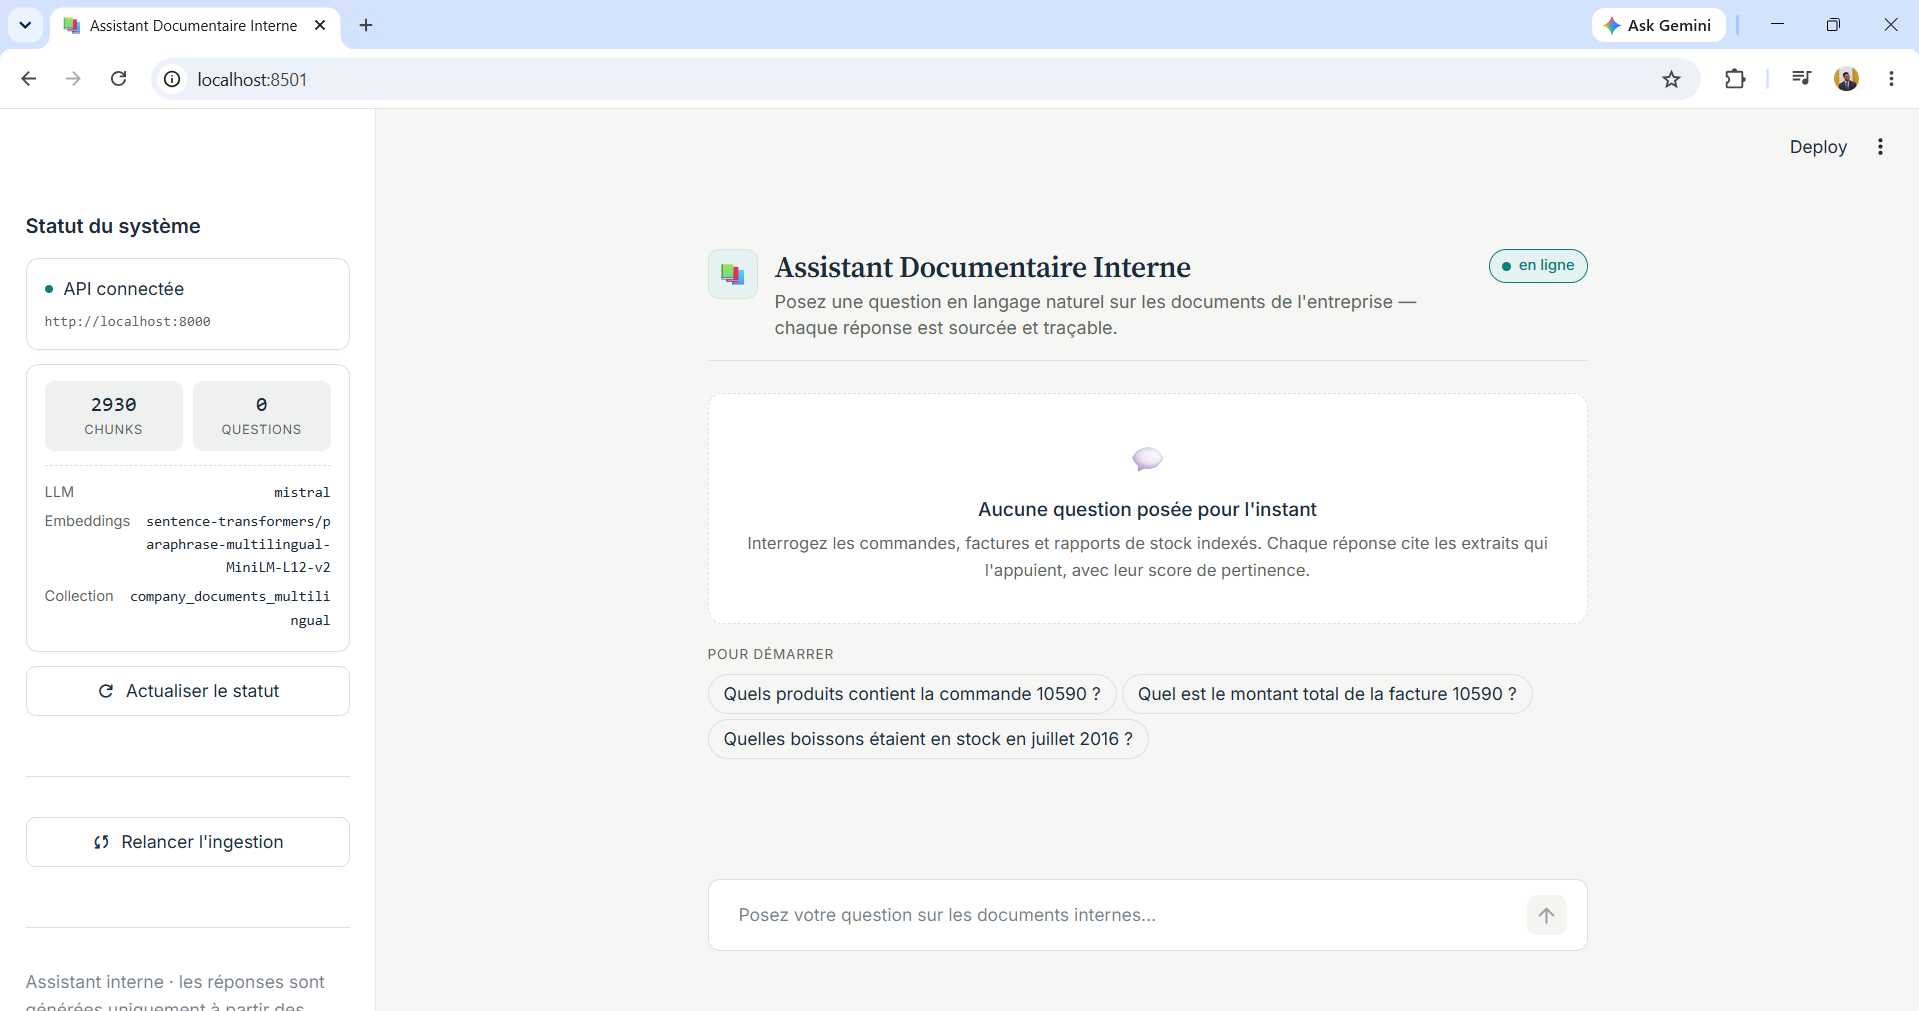
\includegraphics[width=\textwidth]{ui-accueil.png}
\caption{Écran d'accueil de l'assistant. La barre latérale affiche l'état du
système ; la zone centrale propose des questions d'amorçage cohérentes avec le
corpus indexé.}
\label{fig:ui-accueil}
\end{figure}

\subsection{Réponse sourcée}

La figure~\ref{fig:ui-reponse} montre le système en fonctionnement sur une
question réelle. La réponse est structurée, chaque bon de commande étant restitué
avec son identifiant, sa date, le produit concerné, la quantité et le prix
unitaire. Elle se termine par la liste explicite des fichiers sources utilisés.

Au-dessus de la réponse figure une ligne de métadonnées de traçabilité : le
nombre d'extraits mobilisés, le meilleur score de pertinence obtenu et le temps
de génération. Un panneau dépliable « Provenance » donne accès au détail de
chaque extrait, avec son identifiant de segment et une barre indiquant
visuellement son score.

\begin{figure}[htbp]
\centering
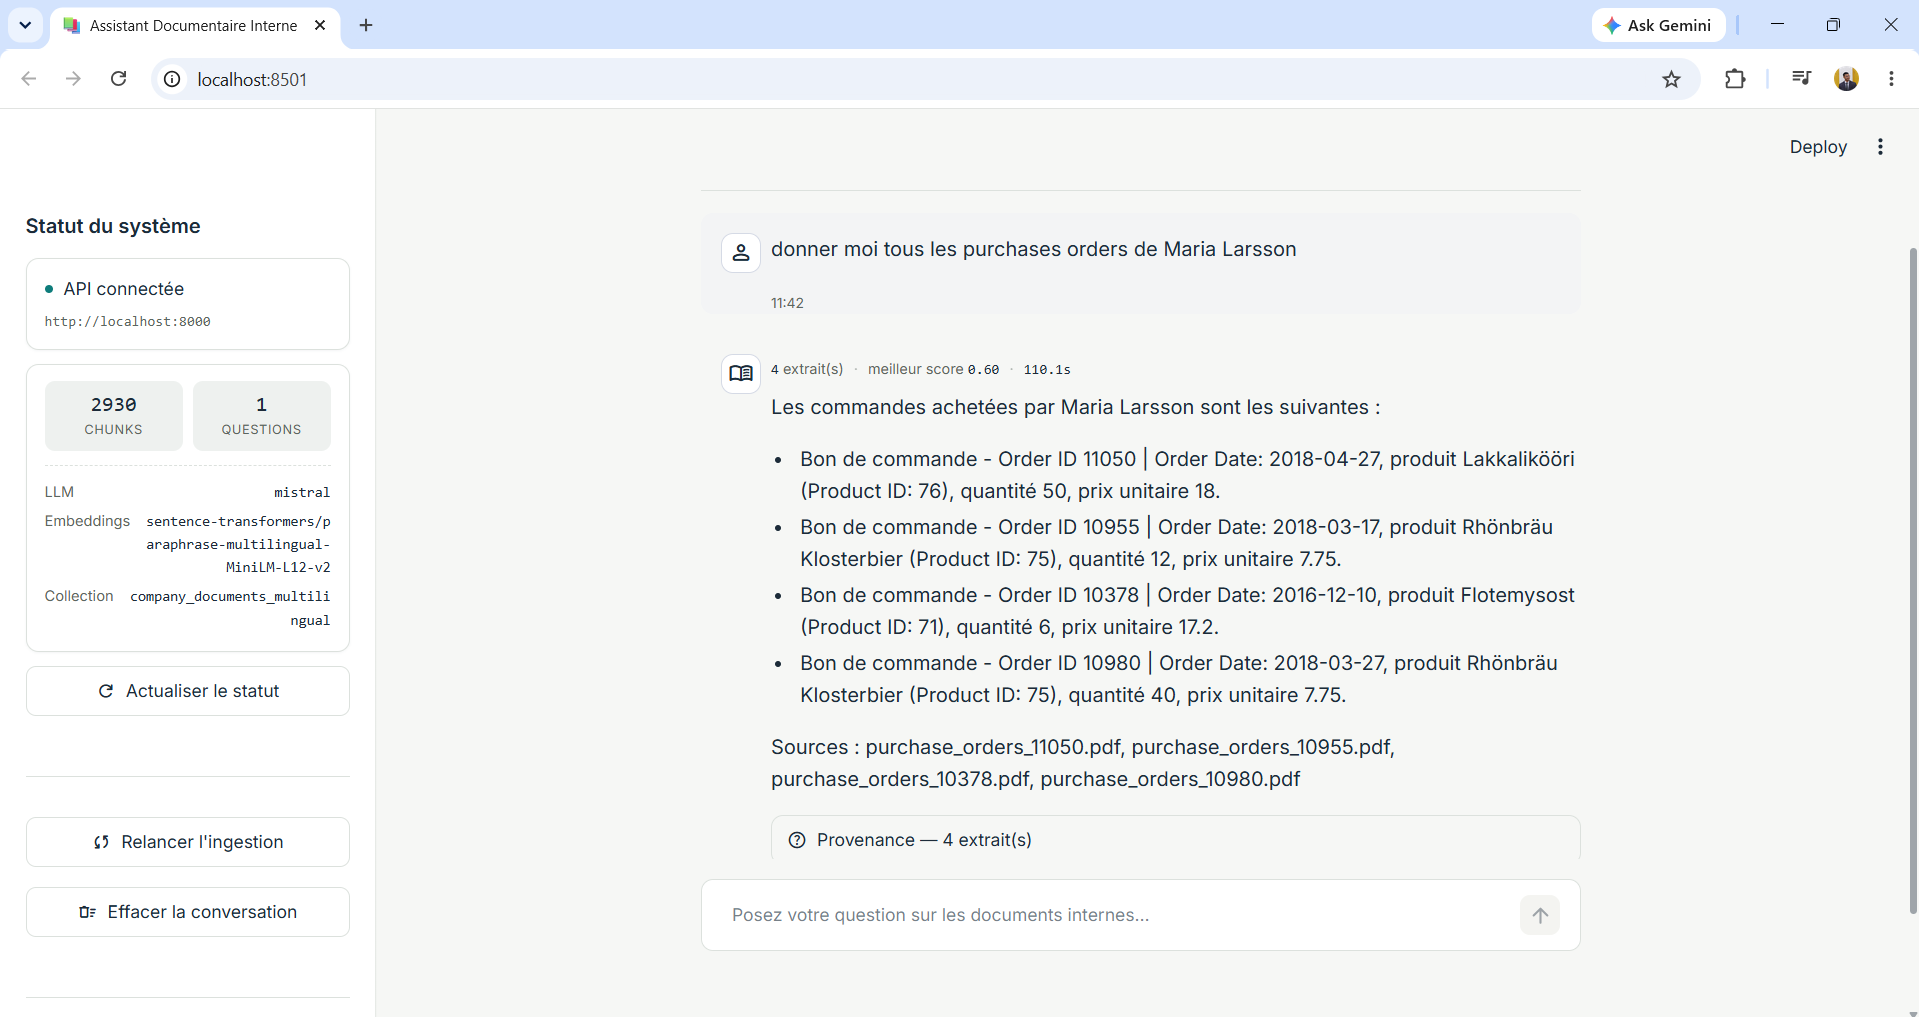
\includegraphics[width=\textwidth]{ui-reponse.png}
\caption{Réponse sourcée produite par le système. Les quatre bons de commande
sont restitués avec leurs détails, suivis de la liste des fichiers sources. La
ligne de métadonnées indique le nombre d'extraits, le meilleur score et le temps
de génération.}
\label{fig:ui-reponse}
\end{figure}

Cet affichage constitue la traduction concrète du critère de traçabilité fixé au
chapitre~\ref{ch:metier}. L'utilisateur n'a pas à croire le système : il peut
ouvrir les fichiers cités et vérifier. C'est ce qui distingue un assistant
exploitable en entreprise d'une démonstration technique.

\section{Conteneurisation avec Docker}

\subsection{Organisation}

Le déploiement repose sur trois services orchestrés par \texttt{docker compose},
décrits au tableau~\ref{tab:services}.

\begin{table}[htbp]
\centering
\caption{Services définis dans \texttt{docker-compose.yml}}
\label{tab:services}
\small
\begin{tabularx}{\textwidth}{@{}p{2.7cm}p{1.5cm}p{3.1cm}X@{}}
\toprule
\textbf{Service} & \textbf{Port} & \textbf{Image} & \textbf{Rôle} \\
\midrule
\texttt{rag-ollama} & 11434 & \texttt{ollama/ollama} &
Sert le modèle Mistral 7B ; volume persistant pour les poids \\
\texttt{rag-api} & 8000 & \texttt{Dockerfile.api} &
Moteur RAG et API REST ; monte \texttt{./data} pour accéder à l'index \\
\texttt{rag-streamlit} & 8501 & \texttt{Dockerfile.streamlit} &
Interface web ; ne connaît que l'URL de l'API \\
\bottomrule
\end{tabularx}
\end{table}

Deux volumes assurent la persistance : \texttt{ollama\_data} conserve les poids
du modèle, évitant un téléchargement de 4,4~Go à chaque redémarrage, et
\texttt{./data} conserve l'index ChromaDB, évitant une ré-ingestion complète.

La configuration inter-services s'effectue par variables d'environnement, les
conteneurs se résolvant par leur nom de service sur le réseau Docker interne :

\begin{lstlisting}[style=plain,caption={Extrait de \texttt{docker-compose.yml}}]
  api:
    build: { context: ., dockerfile: Dockerfile.api }
    container_name: rag-api
    ports: ["8000:8000"]
    environment:
      - OLLAMA_BASE_URL=http://ollama:11434
      - CHROMA_PERSIST_DIR=/app/data/processed/chroma_db
    volumes: ["./data:/app/data"]
    depends_on: [ollama]
\end{lstlisting}

\subsection{Mise en service}

Le déploiement complet tient en deux commandes :

\begin{lstlisting}[style=bash,caption={Déploiement conteneurisé}]
docker compose up --build -d
docker exec -it rag-ollama ollama pull mistral
\end{lstlisting}

La seconde commande télécharge les poids du modèle dans le conteneur Ollama. Elle
n'est nécessaire qu'au premier démarrage, le volume persistant conservant
ensuite le modèle.

L'ingestion du corpus s'effectue alors par simple appel à l'API :

\begin{lstlisting}[style=bash,caption={Ingestion via l'API}]
curl -X POST http://localhost:8000/ingest \
     -H "Content-Type: application/json" \
     -d '{"reset": true}'
\end{lstlisting}

\section{Points de vigilance avant mise en production}

L'état actuel du déploiement est fonctionnel en environnement de développement,
mais plusieurs points doivent être traités avant toute exposition réelle. Ils
sont recensés au tableau~\ref{tab:vigilance} par ordre de criticité.

\begin{table}[htbp]
\centering
\caption{Points de vigilance identifiés}
\label{tab:vigilance}
\small
\begin{tabularx}{\textwidth}{@{}p{4.1cm}p{2.1cm}X@{}}
\toprule
\textbf{Point} & \textbf{Criticité} & \textbf{Action requise} \\
\midrule
Dépendances non figées &
\aremplir{Bloquant} &
Plusieurs modules importés par le code (\texttt{pypdf}, \texttt{python-docx},
\texttt{sentence-transformers}, \texttt{httpx}, \texttt{ragas},
\texttt{datasets}) ne figurent pas dans \texttt{requirements.txt}. La
construction des images Docker produit donc des conteneurs incomplets. Ce
fichier doit être complété et les versions figées \\
\addlinespace
Absence d'authentification & Élevée &
L'API et l'interface n'ont aucun contrôle d'accès. Ajouter une clé d'API ou
OAuth, et placer un \eng{reverse proxy} avec HTTPS devant l'interface \\
\addlinespace
Exposition des services internes & Élevée &
Restreindre l'accès réseau à Ollama et ChromaDB, qui ne doivent pas être
joignables publiquement \\
\addlinespace
Journalisation d'audit & Moyenne &
Tracer qui a posé quelle question et quelles sources ont été mobilisées, à des
fins de conformité \\
\addlinespace
Filtrage des documents sensibles & Moyenne &
Anonymiser ou exclure les documents à caractère personnel avant ingestion
(RGPD) \\
\addlinespace
Latence de génération & Moyenne &
Prévoir un GPU ou un modèle quantifié pour un usage quotidien
(\emph{cf.} chapitre~\ref{ch:evaluation}) \\
\bottomrule
\end{tabularx}
\end{table}

Le premier point mérite un commentaire. Il illustre un écueil classique du
développement : l'environnement local a été enrichi progressivement par
installations successives, sans que le fichier de dépendances soit tenu à jour.
Le code fonctionne donc parfaitement sur la machine de développement tout en
étant irreproductible ailleurs --- ce qui est précisément ce que la
conteneurisation est censée éliminer. La leçon est de valider systématiquement
une construction depuis un environnement vierge, et non depuis l'environnement de
travail.

\section{Versionnement}

Le code source est versionné avec Git. L'arborescence du projet sépare
explicitement les responsabilités, comme le montre le
listing~\ref{lst:arbo}.

\begin{lstlisting}[style=plain,caption={Organisation du dépôt},label={lst:arbo}]
rag-enterprise-assistant/
|-- src/
|   |-- config.py              # configuration centralisee (.env)
|   |-- ingestion/             # chargement, decoupage, indexation
|   |-- rag/                   # recherche, generation, pipeline
|   |-- evaluation/            # metriques RAGAS
|   |-- api/                   # backend FastAPI
|   +-- app/                   # interface Streamlit
|-- scripts/ingest_documents.py
|-- data/
|   |-- raw/                   # corpus source
|   |-- processed/             # index ChromaDB persiste
|   +-- eval/testset.csv       # jeu d'evaluation
|-- tests/
|-- docs/                      # architecture, guide de deploiement
|-- Dockerfile.api
|-- Dockerfile.streamlit
|-- docker-compose.yml
|-- Makefile
+-- requirements.txt
\end{lstlisting}

Un \texttt{Makefile} centralise les opérations courantes
(\texttt{make ingest}, \texttt{make api}, \texttt{make ui}, \texttt{make eval},
\texttt{make test}), ce qui réduit le risque d'erreur de manipulation et
documente de fait les commandes utiles du projet.

\section{Conclusion}

Ce chapitre a présenté le déploiement du système en trois services conteneurisés :
un serveur de modèle Ollama, une API REST FastAPI exposant quatre
\eng{endpoints}, et une interface conversationnelle Streamlit. Le découplage
strict entre l'interface et le moteur permet de substituer l'une sans toucher à
l'autre. Les captures présentées attestent du fonctionnement effectif de la
chaîne complète, de la question posée jusqu'à la réponse sourcée accompagnée de
ses extraits et de leurs scores. Les points de vigilance à traiter avant une
exposition réelle ont été recensés, le plus critique étant la complétion du
fichier de dépendances.
